%%% template.tex
%%%
%%% This LaTeX source document can be used as the basis for your technical
%%% paper or abstract. Intentionally stripped of annotation, the parameters
%%% and commands should be adjusted for your particular paper - title, 
%%% author, article DOI, etc.
%%% The accompanying ``template.annotated.tex'' provides copious annotation
%%% for the commands and parameters found in the source document. (The code
%%% is identical in ``template.tex'' and ``template.annotated.tex.'')

\documentclass[conference, 12pt]{acmsiggraph}

\title{Interactive Crowd Simulation guided by a Kinect Sensor User Interface}

\author{Grant Adam Mulitz-Schimel \and Lu Yang \and Rafael Farias Marinheiro \and Sam Luo Nelson \and Tae Hoon Kim}
% \contactemail{}
\affiliation{Cornell University\thanks{\{gam244, ly77, rf356, sln58, tk536\}@cornell.edu}}
\pdfauthor{Rafael F. Marinheiro}

\keywords{crowd simulation, user interaction, real-time rendering}

\usepackage{amsmath}


\begin{document}

%% \teaser{
%%   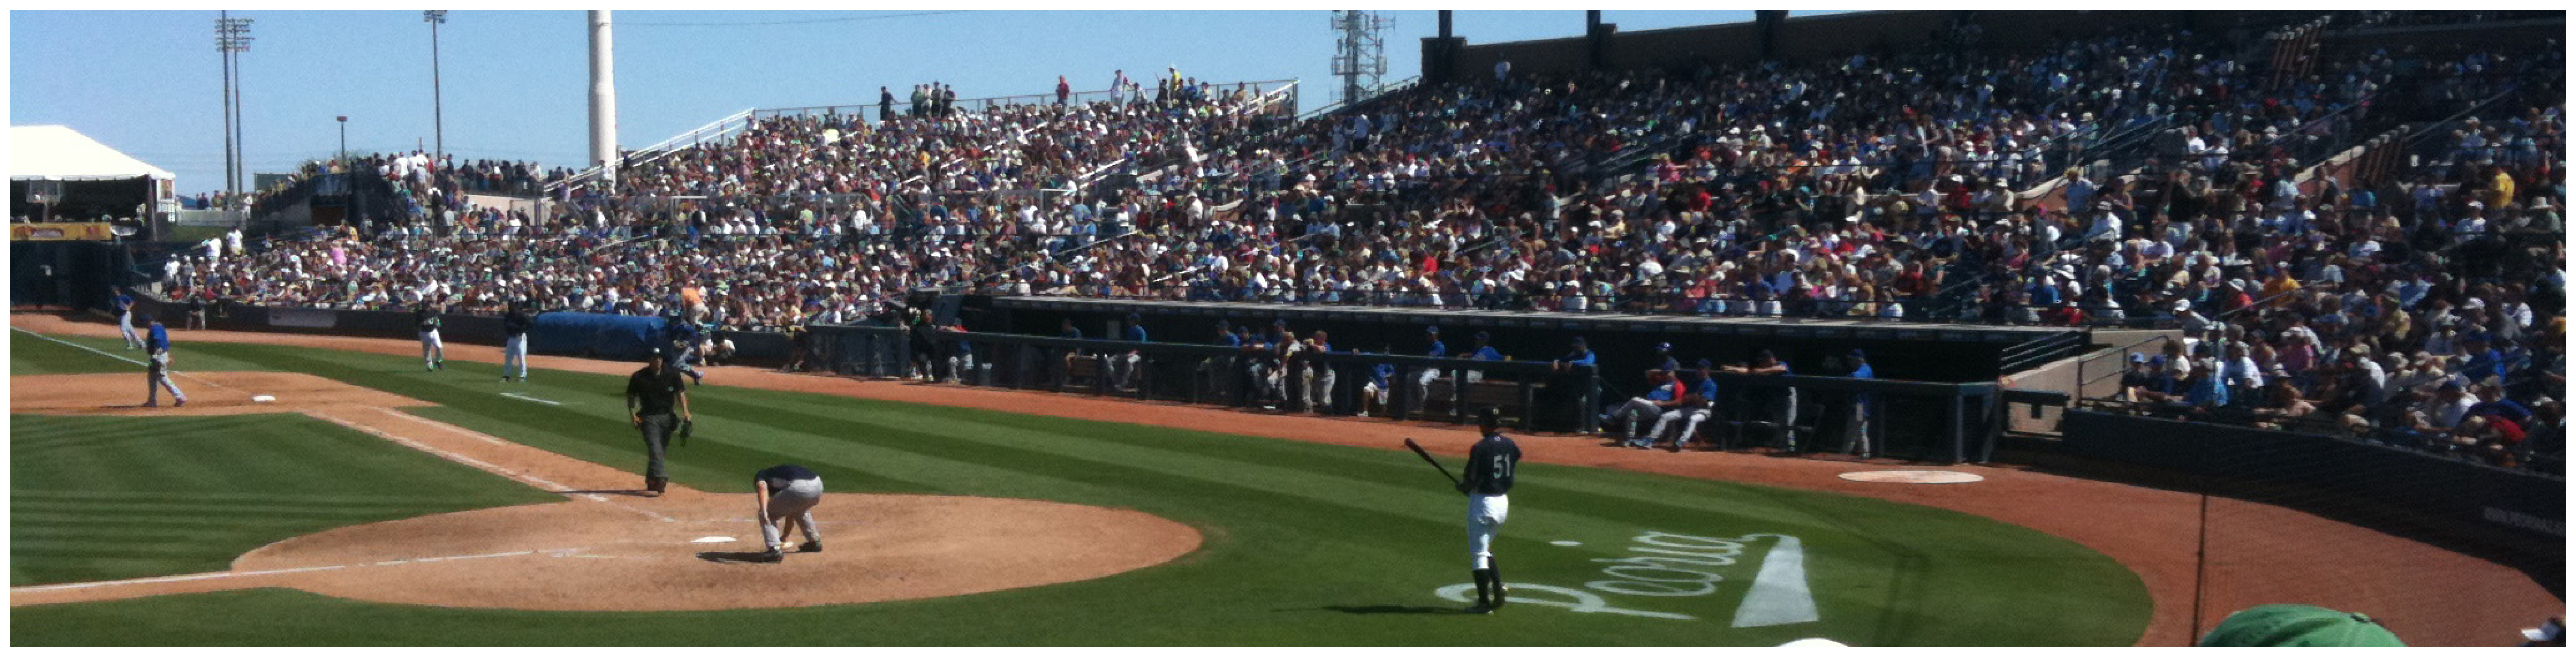
\includegraphics[height=1.5in]{images/sampleteaser}
%%   \caption{Spring Training 2009, Peoria, AZ.}
%% }

\maketitle

\begin{abstract}

We intend to create a interactive Crowd Simulation application using the approach described in \cite{kim2012interactive}. The user will be able to interact with the application with a commodity depth sensor \cite{Zhang:2012:MKS:2225053.2225203}, modifying the environment in real time.

\end{abstract}

\begin{figure}[Ht!]
  \centering
    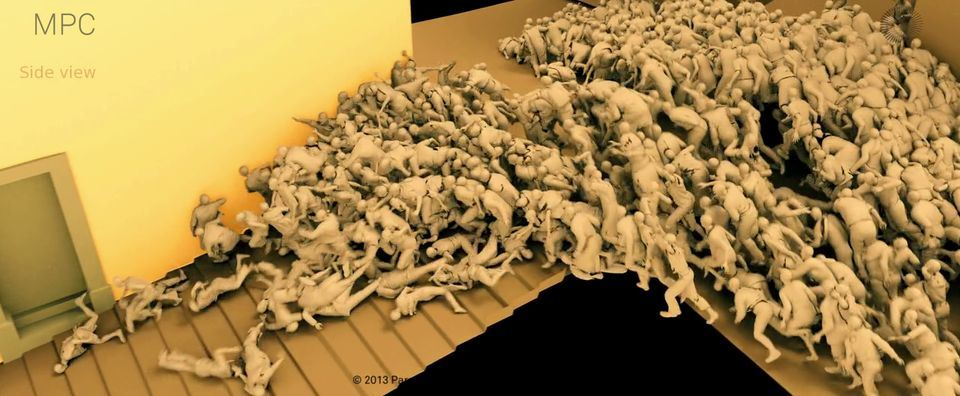
\includegraphics[width=0.5\textwidth]{images/mpc3.jpg}
    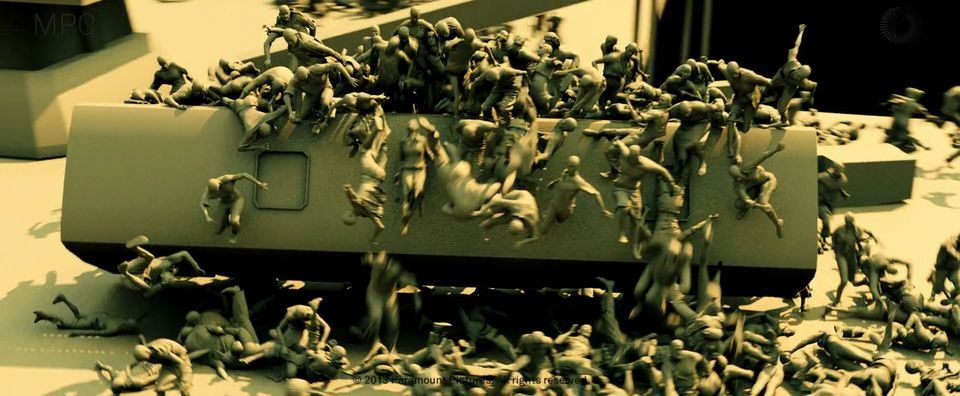
\includegraphics[width=0.5\textwidth]{images/mpc2.jpg}
	\caption{World War Z (2013). Zombie agents were computationally simulated.}
	\label{fig:wwz}
\end{figure}

%% Use this only if you're preparing a technical paper to be published in the 
%% ACM 'Transactions on Graphics' journal.

\begin{CRcatlist}
	\CRcat{I.2.11}{Artificial Intelligence}{Distributed Artificial Intelligence}{Multiagent systems};
	\CRcat{I.3.7}{Computer Graphics}{Three-Dimensional Graphics and Realism}{Animation};
	\CRcat{I.6.8}{Simulation and Modeling}{Types of Simulation}{Animation}
\end{CRcatlist}

%%% The ``\keywordlist'' prints out the user-defined keywords.

\keywordlist

\TOGlinkslist

%% Required for all content. 

\copyrightspace

\section{Overview}

When trying to create highly detailed virtual environments, such as those present in movies and games, it is necessary to add extra elements to the scene to enrich the user experience. One important element that is almost always present in modern virtual environments is the crowd: a set of agents that are part of the scene and that must behave according to the environment.

In interactive applications, such as in games, the crowd must behave according to the user's actions. Therefore, the application must simulate the behavior of those agents in runtime. In non-interactive applications, such as in movies, the artists have the freedom to create the scene beforehand. However, when trying to create large scale scenes, it is unpractical to use artists to model every agent, so the director may choose to use computational methods to create the scene (see Figure \ref{fig:wwz}).

\section{Software Deliverable}
	We will deliver a interactive Crowd Simulation application. The user will be able to interact with the agents of the Crowd by using a Kinect Sensor. He will be able to assign orders to the crowd and also to modify the environment (by throwing fireballs, modifying the terrain, adding obstacles and so on).

\section{Techniques}
In order to implement the Crowd Simulation, we will use the Crowd Simulation method described in \cite{kim2012interactive}. This method allows the user to add special elements called Stressors, that affect directly the way that agents choose their path.

We intend to use Microsoft Kinect Sensor to allow the user to interact directly with the crowd. To add realism to the scene, we intend to use modern Real-Time rendering techniqe such as Deferred Shading \cite{hargreaves2004deferred}, Shadow Mapping \cite{Stamminger:2002:PSM:566654.566616} and etc.

The software will be implemented using C++ and OpenGL.

\section{Software Architecture}

We will split this project in 3 different modules.

\subsection{Crowd Simulation}
This module is responsible for controlling the behavior of the agents. Grant and Lu will work in this module.

\subsection{Rendering}
This module is responsible for rendering the virtual environment to the user. Rafael and Sam will work in this module.

\subsection{User Interaction}
This module is responsible for managing the input data that comes from the Kinect Sensor. Tae will work in this module.

\section{Milestones}

We intend to complete each module separately by the first Milestone (November 14th). After that, we will start to integrate all theses modules together into a single application, which will be presented by the end of the course.


\bibliographystyle{acmsiggraph}
\bibliography{proposal}
\end{document}
